\section{Edit package sources}\subsection{Information}
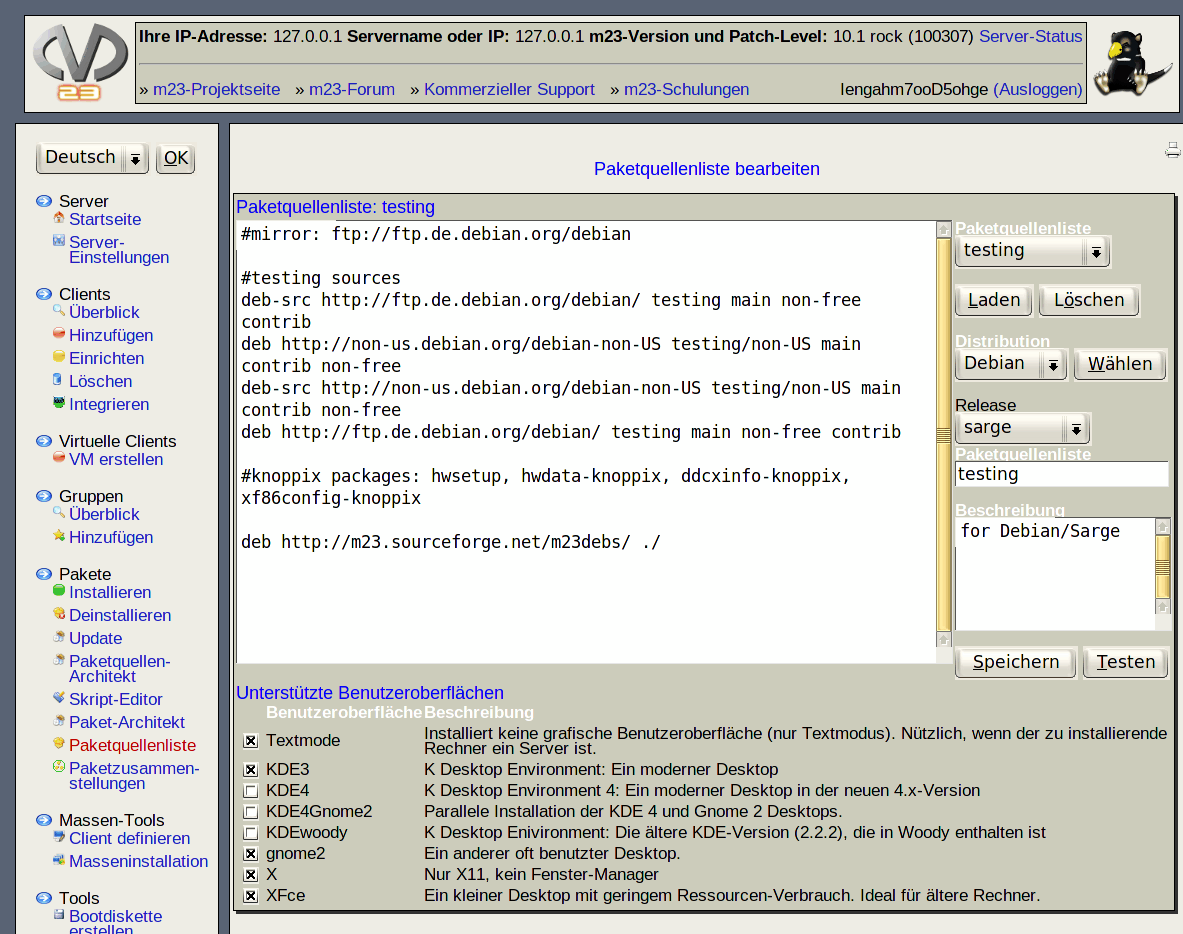
\includegraphics[scale=0.4]{/mdk/doc/manual/screenshots/en/client_sourceslist.png} \\
Software packages can be installed from different sources (HTTP,FTP,CDRom etc.). Different sources are needed, if not all of the software packages can be installed from the same medium. To make it easy for you to administrate these package sources, you can enter them as expected by your selected distribution.\\
\begin{itemize}
	\item \textbf{Loading a package source}: Select a package source from the list (top/right) and click on \textit{"Load"}. The package source will be loaded in the editor.\\
	\item \textbf{Deletion a package source}: To delete the package source loaded in the editor, click on the \textit{"Delete"} button and accept your decision in the next dialog.\\
	\item \textbf{Saving a package source}: The system will always save the package source loaded in the editor. It doesn't matter which package source is selected in the list. Think about a good name for your package source and enter it below \textit{"Pool name"}. If you have loaded a package source before, the package source name is written into the field \textit{"Pool name"} automatically. If you want, you can enter a comment into the \textit{"Description"} text field. Afterwards, click on the \textit{"Save"} button.\\
	\item \textbf{Test the package source}: After entering a package source list, you should test if all sources are working properly. Simply click on the \textit{"Test"} button. The package description files will be downloaded and a test report will be shown thereafter. It can take minutes until the report is shown, depending on your internet connection speed and the speed of the used software package servers.\\
	\item \textbf{Select Mirror}: If you would like to use a different mirror (the standard server is ftp.debian.org) for the installation of the base system, enter it as follows in a new line of your package source: \\
\begin{verbatim}
#mirror: [URL to the packages]
\end{verbatim}
. \textit{URL to the packages} describes the protocol, the hostname or the IP and the directory that contains the packages. A valid URL may look like this: \\
\begin{verbatim}
#mirror: http://192.168.7.14/debianCDs
\end{verbatim}
.\\
\end{itemize}
\subsection{Hint}
\begin{itemize}
\item If you save a package source under a name that already exists, the old package source will be overwritten with the contents of the editor.\\
\item \textbf{Benutzeroberfl�chen} sind direkt an eine Paketquellenliste gebunden. D.h. wenn Sie eine bestimmte Paketquellenliste f�r einen Client benutzen, k�nnen Sie nur die Benutzeroberfl�chen verwenden, die Sie in diesem Dialog f�r die Paketquellenliste freigeschaltet haben. Sie sollten hier deshalb nur die Benutzeroberfl�chen ausw�hlen, die garantiert von den Paketquellen unterst�tzt werden.\\
\end{itemize}
